\chapter{Experimental results}
\indent
	Experiments of this chapter are done with setup below: 
	\begin{itemize}
		\item Seed: 42.
		\item Batch size: 64 (ResNet-18)/16 (ResNet-50).
		\item Number of epochs: 20 (ResNet-18)/10 (ResNet-50).
		\item Learning rate: $10^{-3}$.
		\item Optimizer: \code{SGD} with momentum 0.9 and weight decay $5 \times 10^{-4}$.
	\end{itemize} 

\section{Accuracy and loss}
\indent
	From Figures \ref{resnet18-acc} and \ref{resnet50-acc}, we can see that the models without pretrained does not work, since
	the accuracy does not improve through training. Loss is the same (See Figures \ref{resnet18-loss} and \ref{resnet50-loss}). \\ 
	The best accuracy of ResNet-18 is about \textbf{87\%} for training and \textbf{84\%} for testing, and ResNet-50 is about
	\textbf{86\%} for training and \textbf{85\%} for testing. \\
	\textbf{ResNet-50} is a little bit better for \textbf{testing-accuracy} of this task.

	\begin{figure}[H]
		\centering
		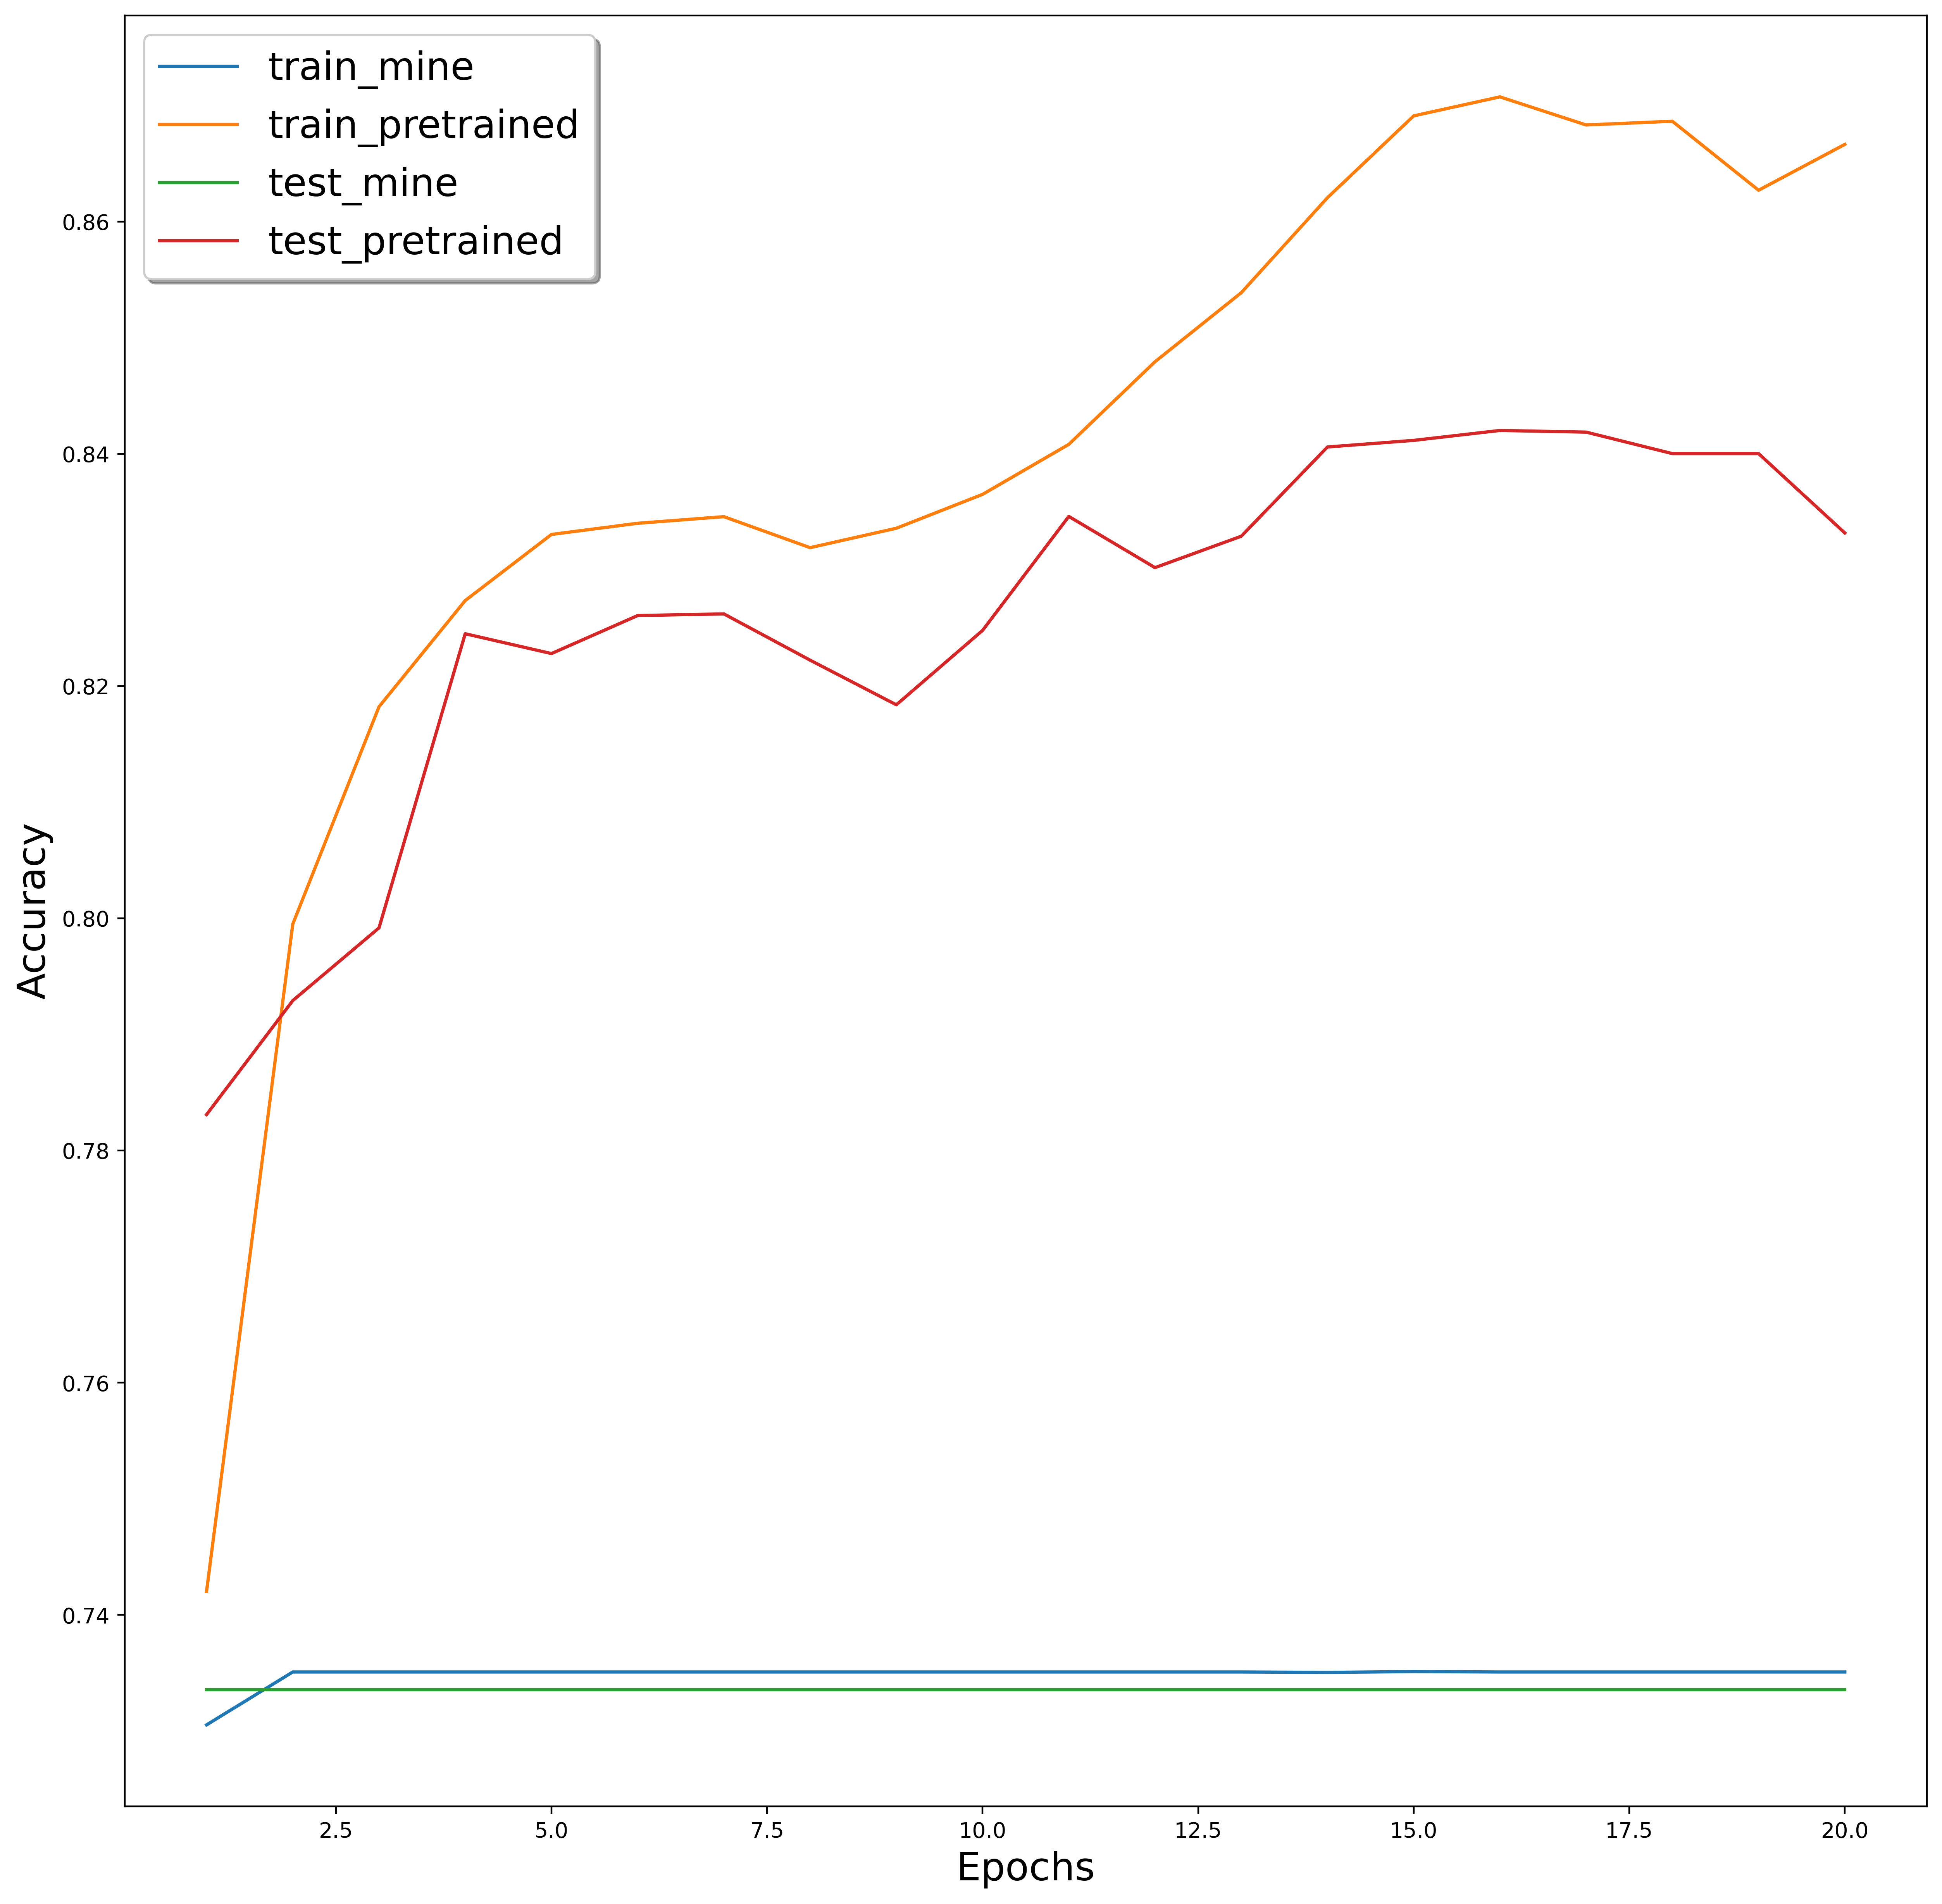
\includegraphics[scale=0.3]{img/resnet18_acc.png}
		\caption{Accuracy of ResNet-18 (with and without pretrained).}
		\label{resnet18-acc}
	\end{figure}
	\begin{figure}[H]
		\centering
		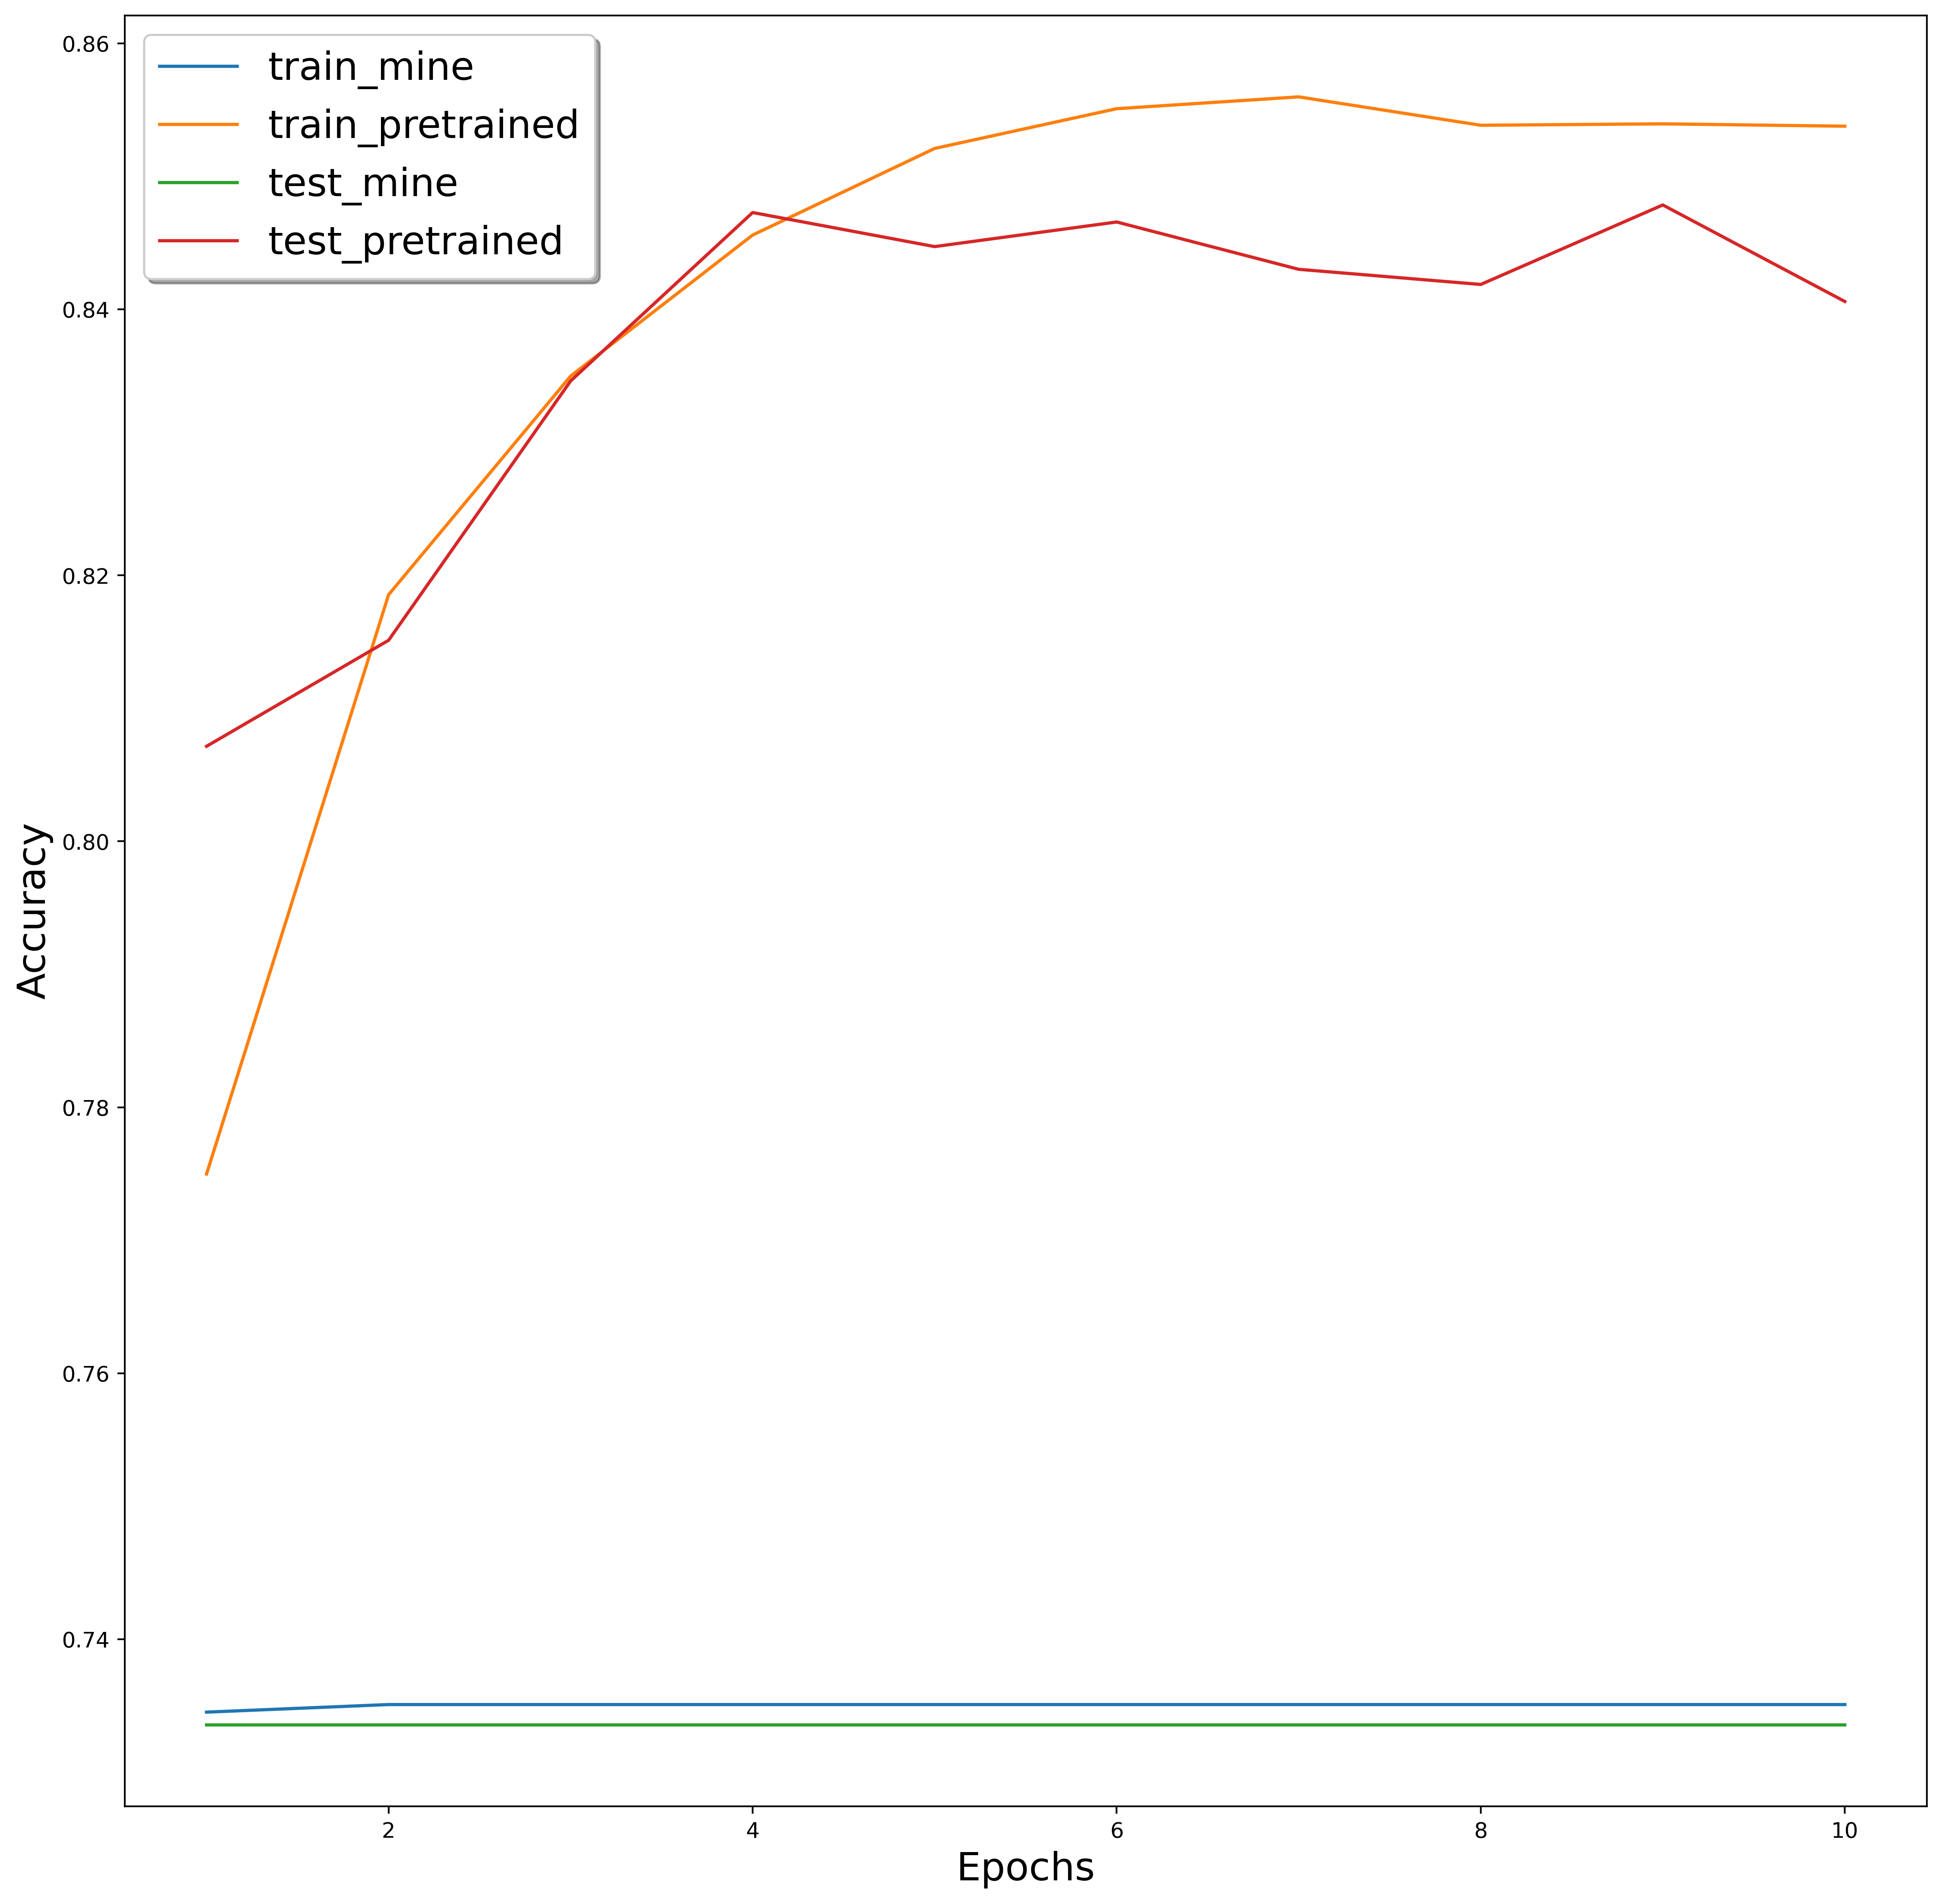
\includegraphics[scale=0.3]{img/resnet50_acc.png}
		\caption{Accuracy of ResNet-50 (with and without pretrained).}
		\label{resnet50-acc}
	\end{figure}

	\begin{figure}[H]
		\centering
		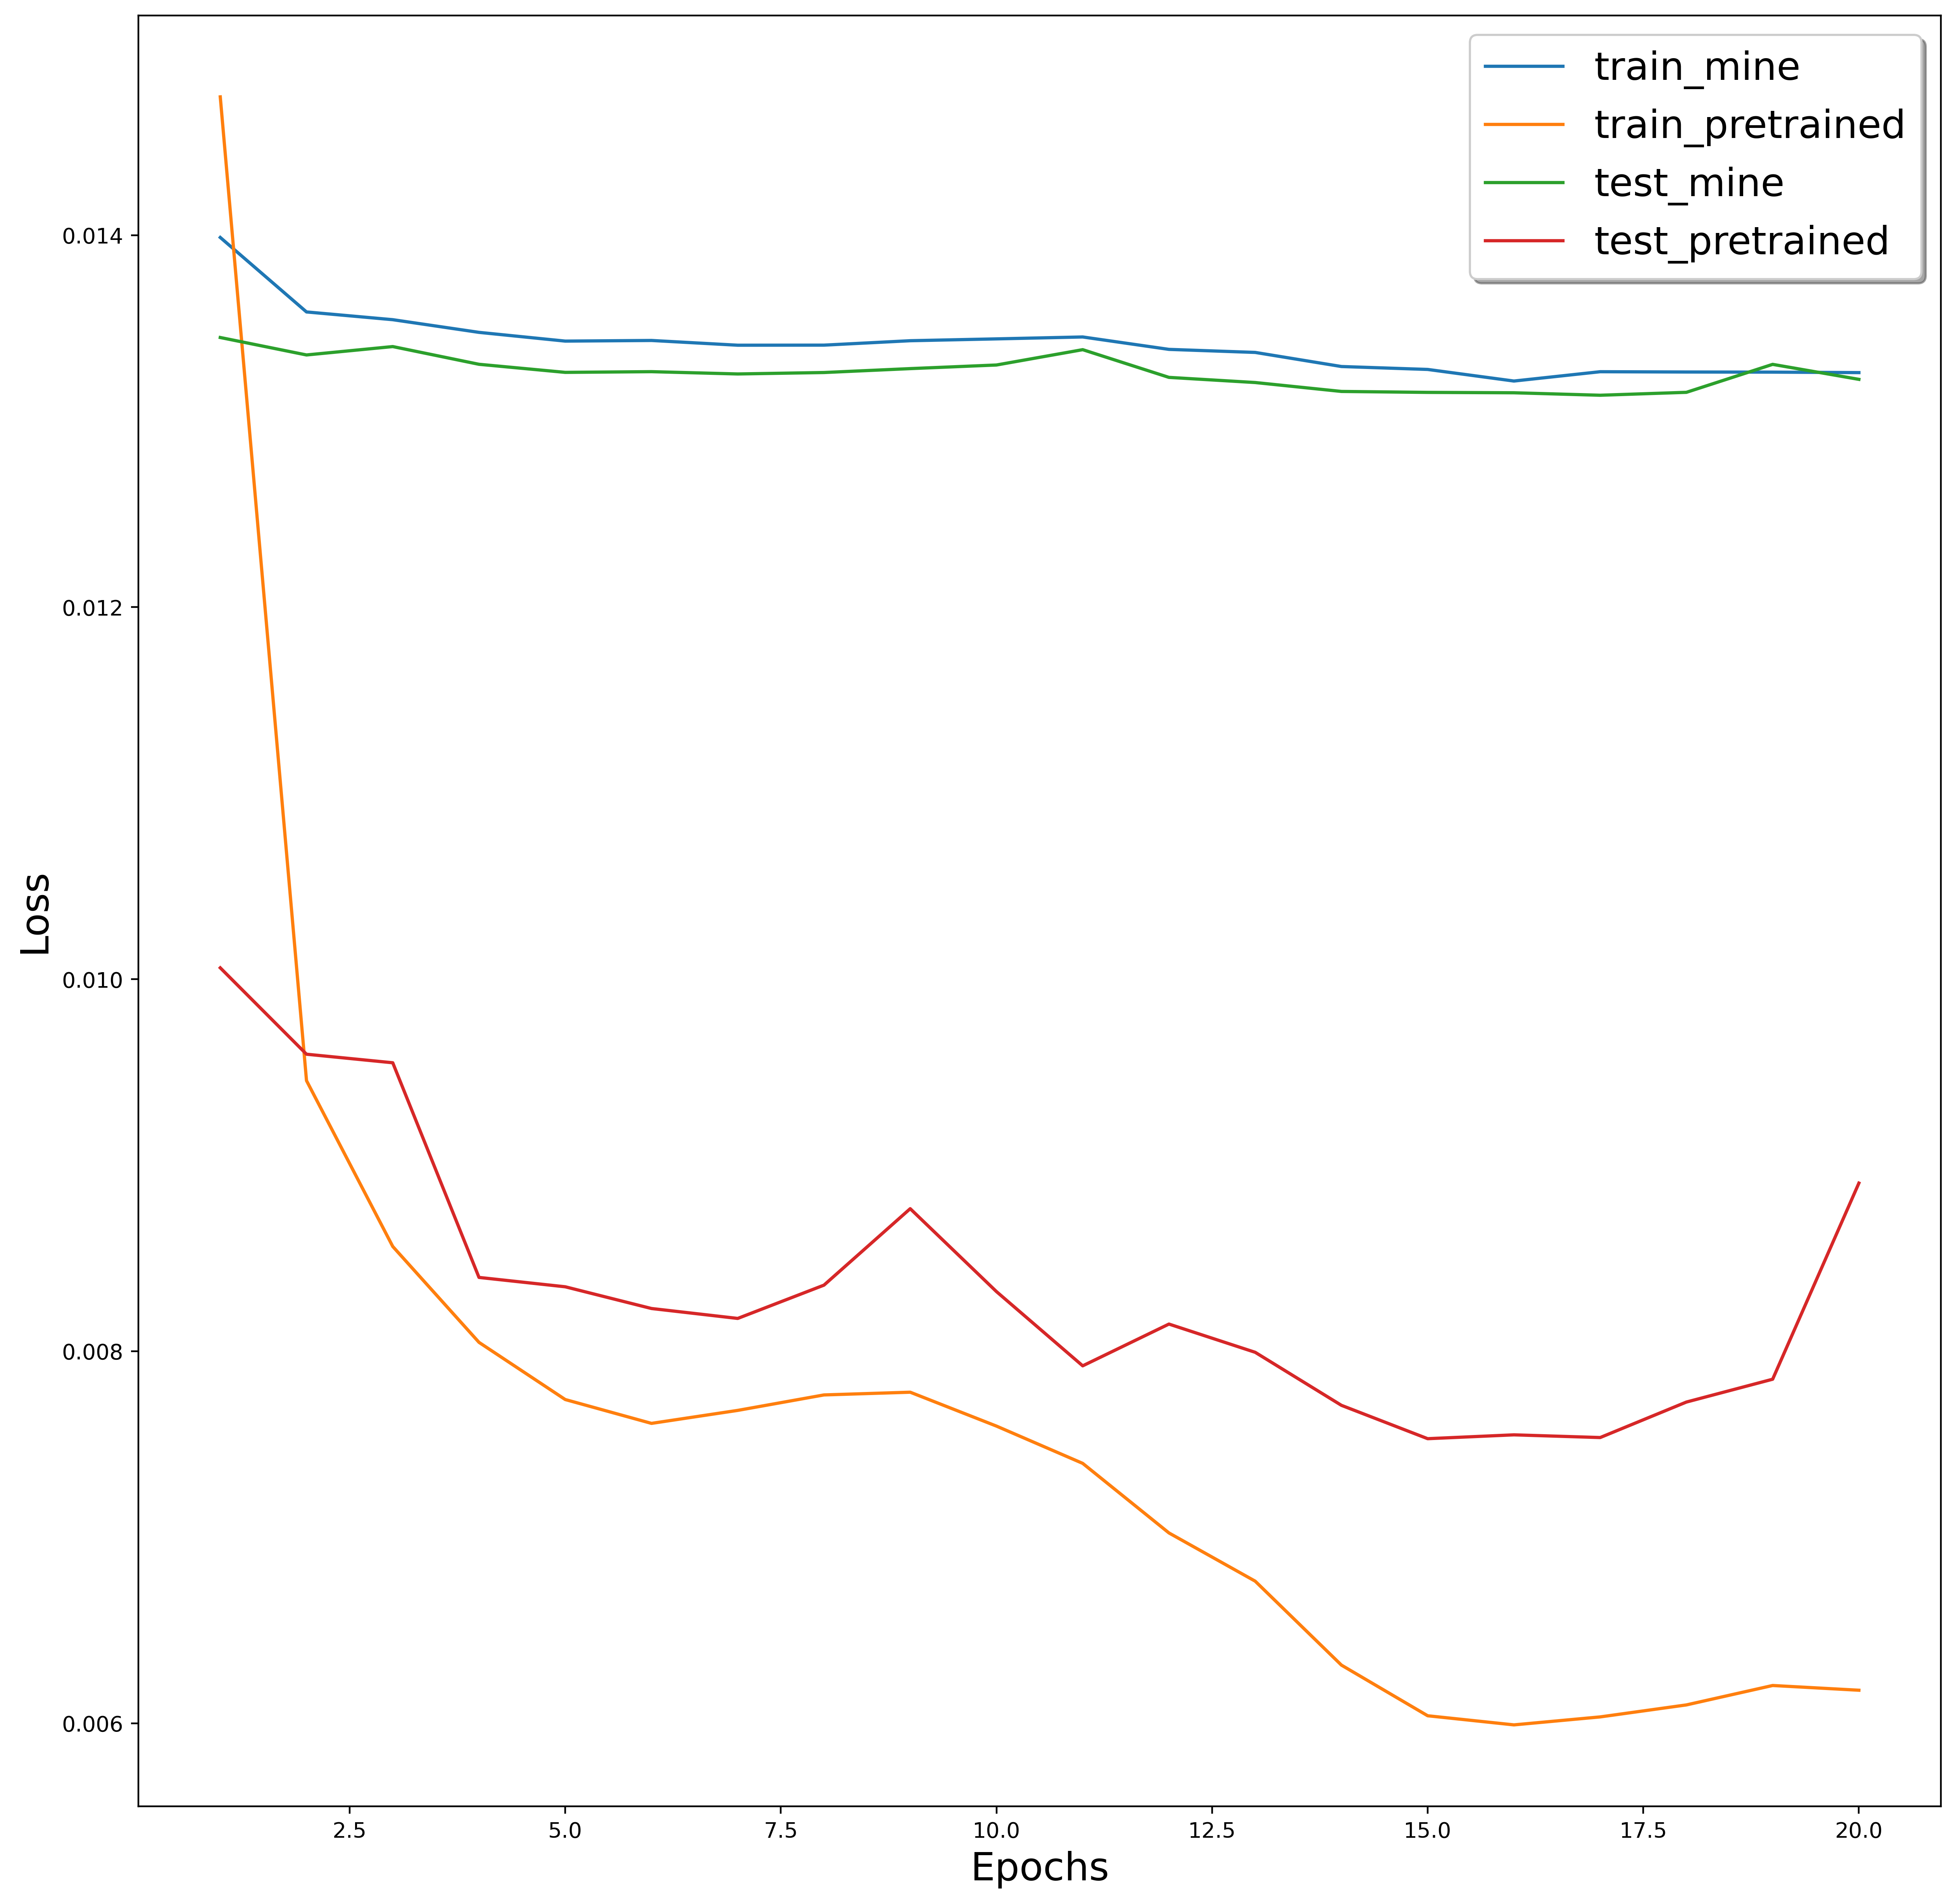
\includegraphics[scale=0.3]{img/resnet18_loss.png}
		\caption{Loss of ResNet-18 (with and without pretrained).}
		\label{resnet18-loss}
	\end{figure}
	\begin{figure}[H]
		\centering
		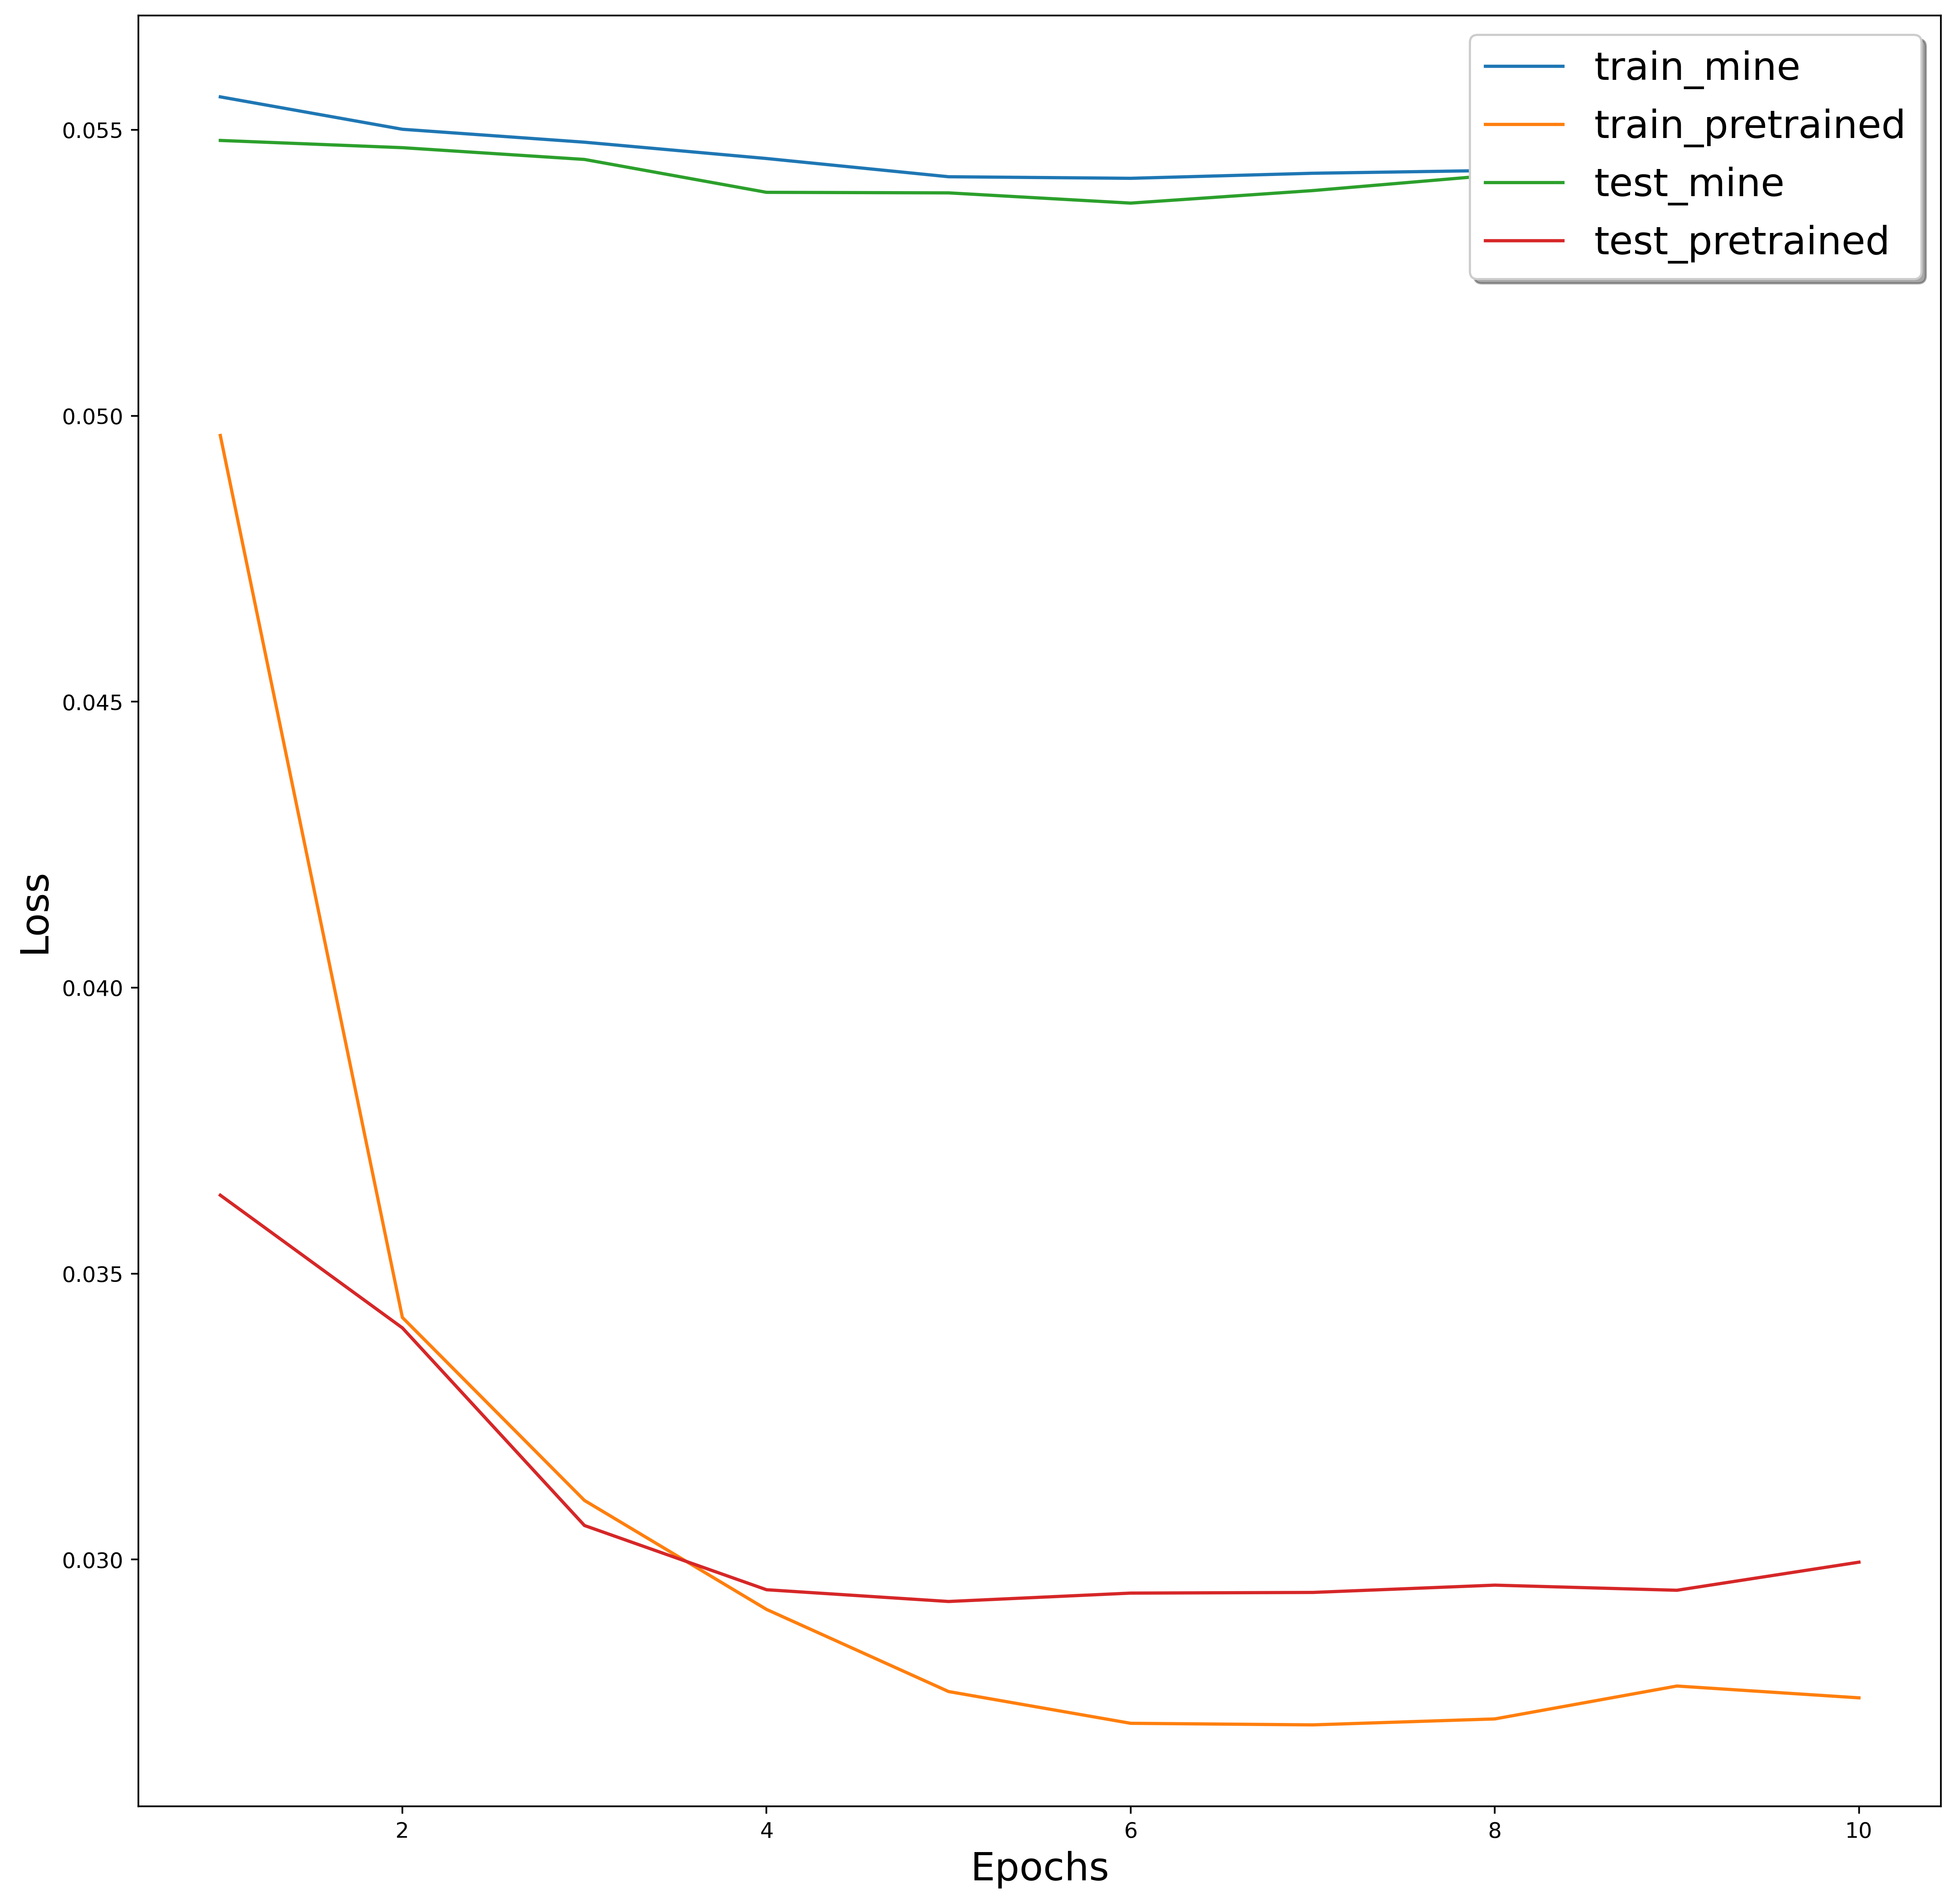
\includegraphics[scale=0.3]{img/resnet50_loss.png}
		\caption{Loss of ResNet-50 (with and without pretrained).}
		\label{resnet50-loss}
	\end{figure}

\section{Confusion matrix}
\indent
	From Figures \ref{resnet18-mine-confusion-matrix} and \ref{resnet50-mine-confusion-matrix}, we can see that the model without pretrained does not work, 
	it's same as previous section, the accuracy does not improve, the loss does not decrease, and the confusion matrices are obviously bad. \\
	And the confusion matrices of pretrained models are much better (See Figures \ref{resnet18-pretrained-confusion-matrix} and \ref{resnet50-pretrained-confusion-matrix}), but 
	also not good enough, since the percentage of correct labels is still not dominant.

	\begin{figure}[H]
		\centering
		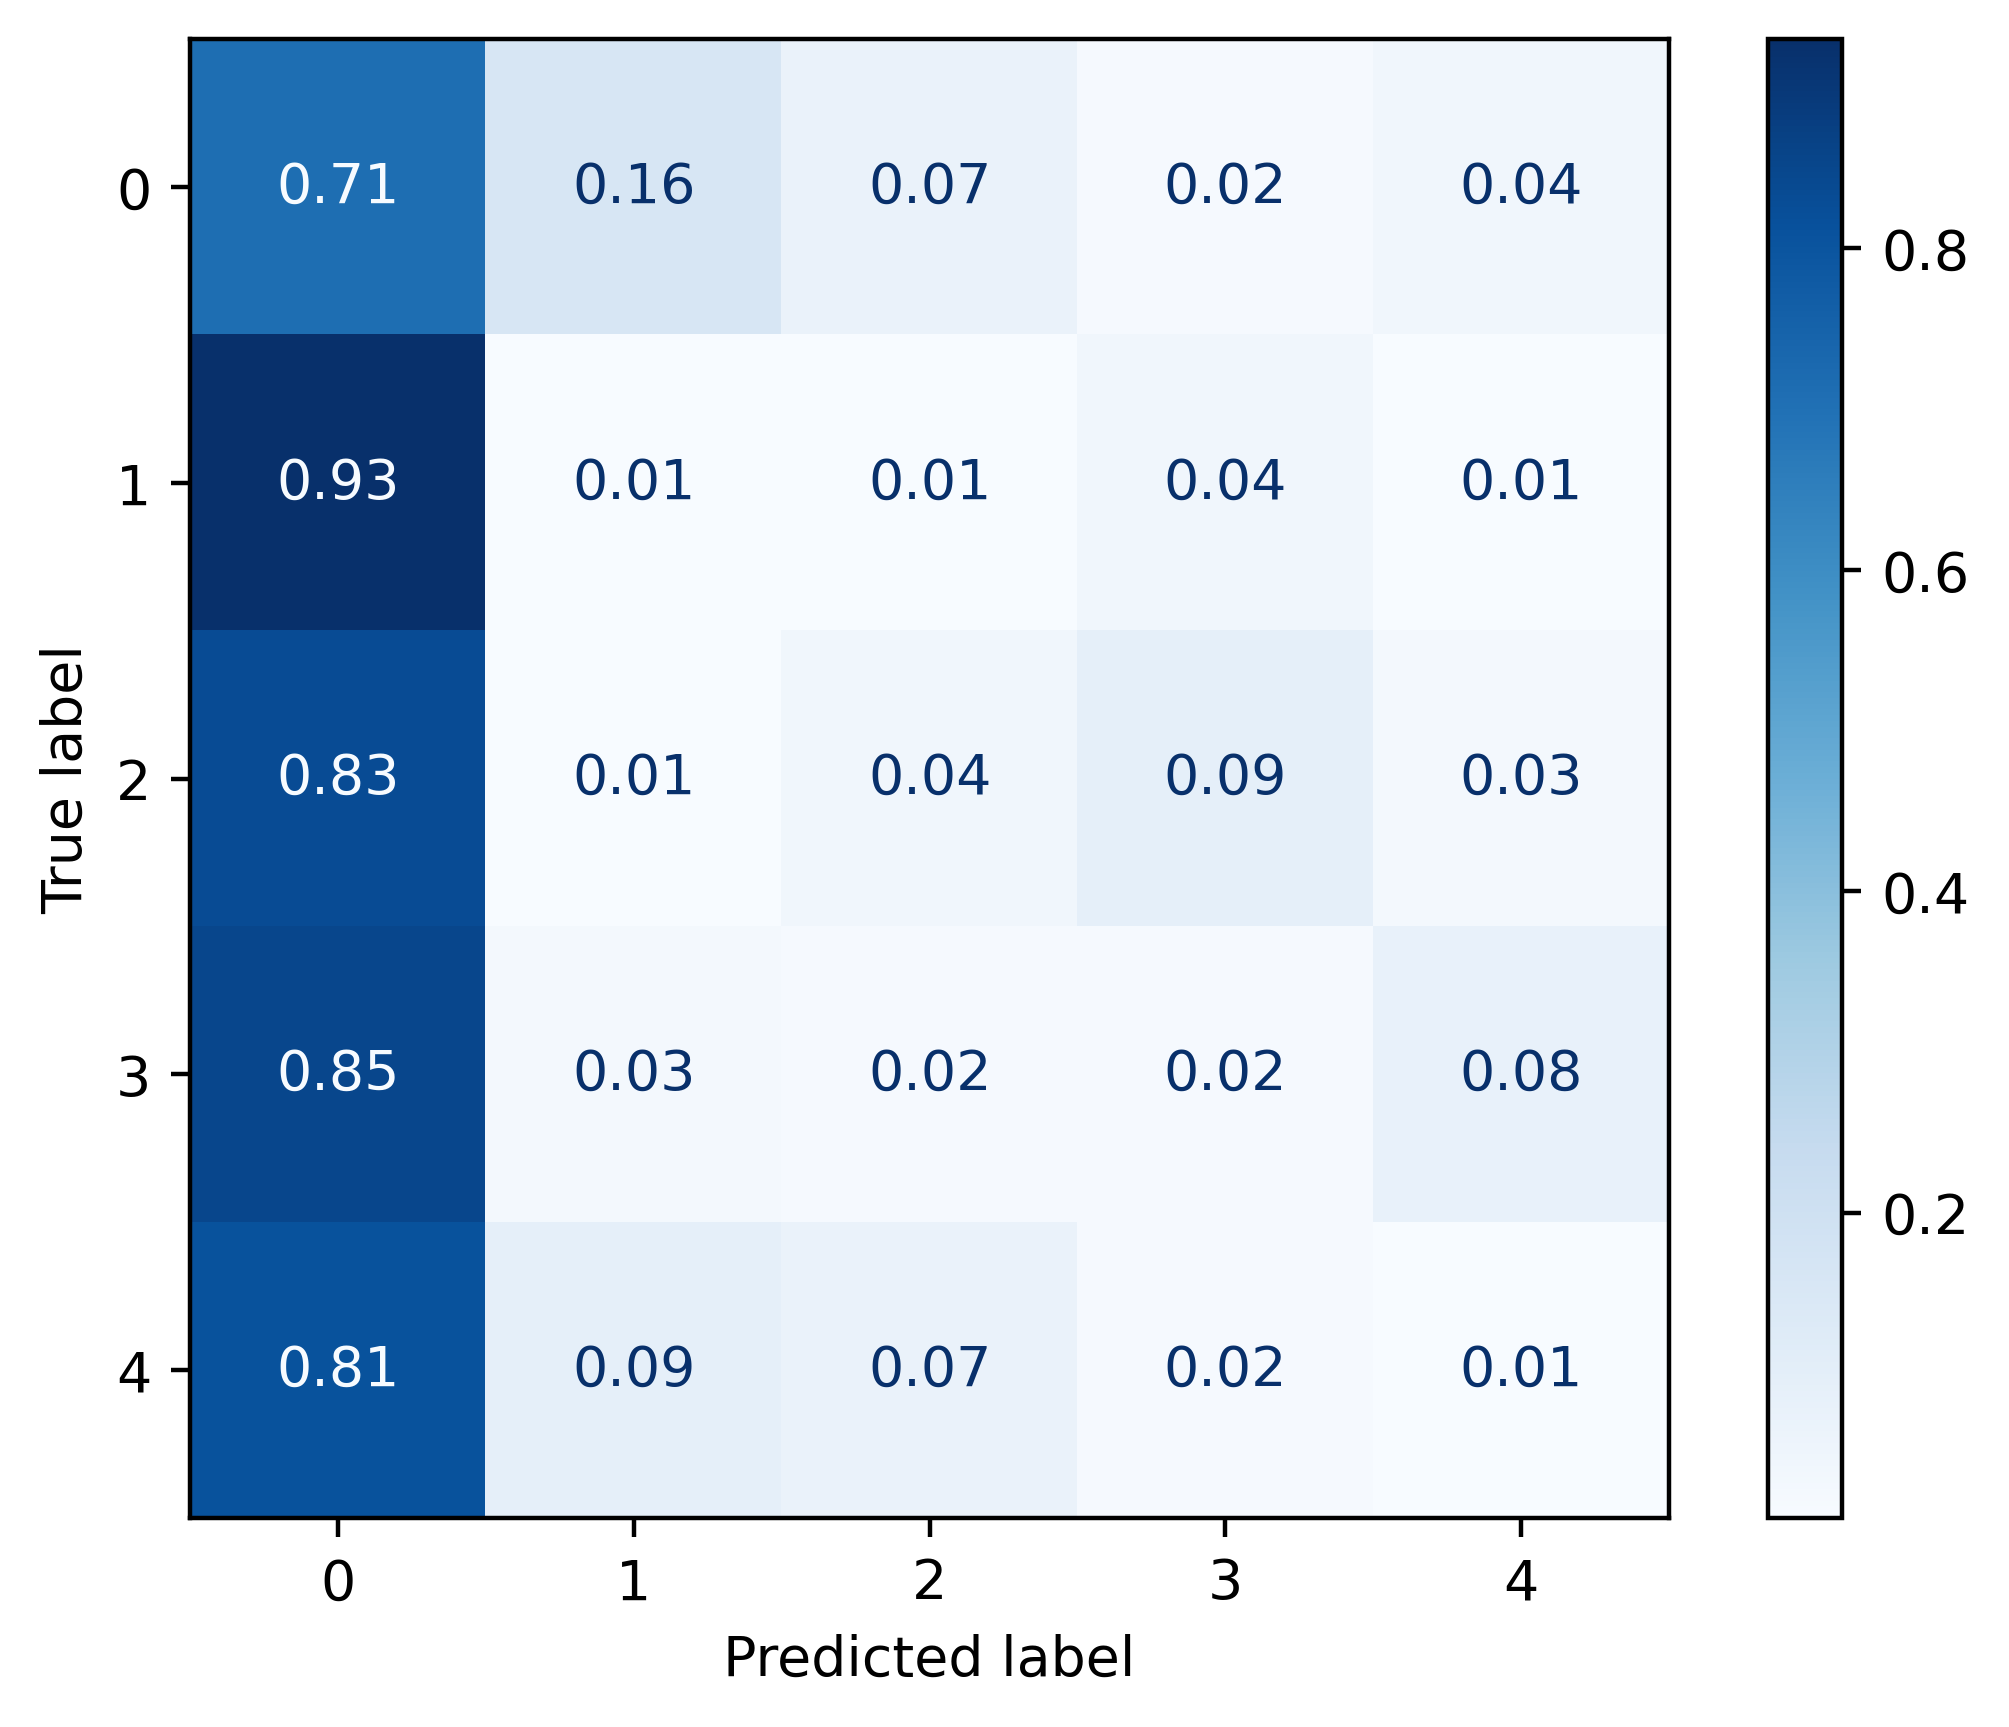
\includegraphics[scale=0.8]{img/resnet18_confusion_matrix_mine.png}
		\caption{Confusion matrix of ResNet-18 (without pretrained).}
		\label{resnet18-mine-confusion-matrix}
	\end{figure}
	\begin{figure}[H]
		\centering
		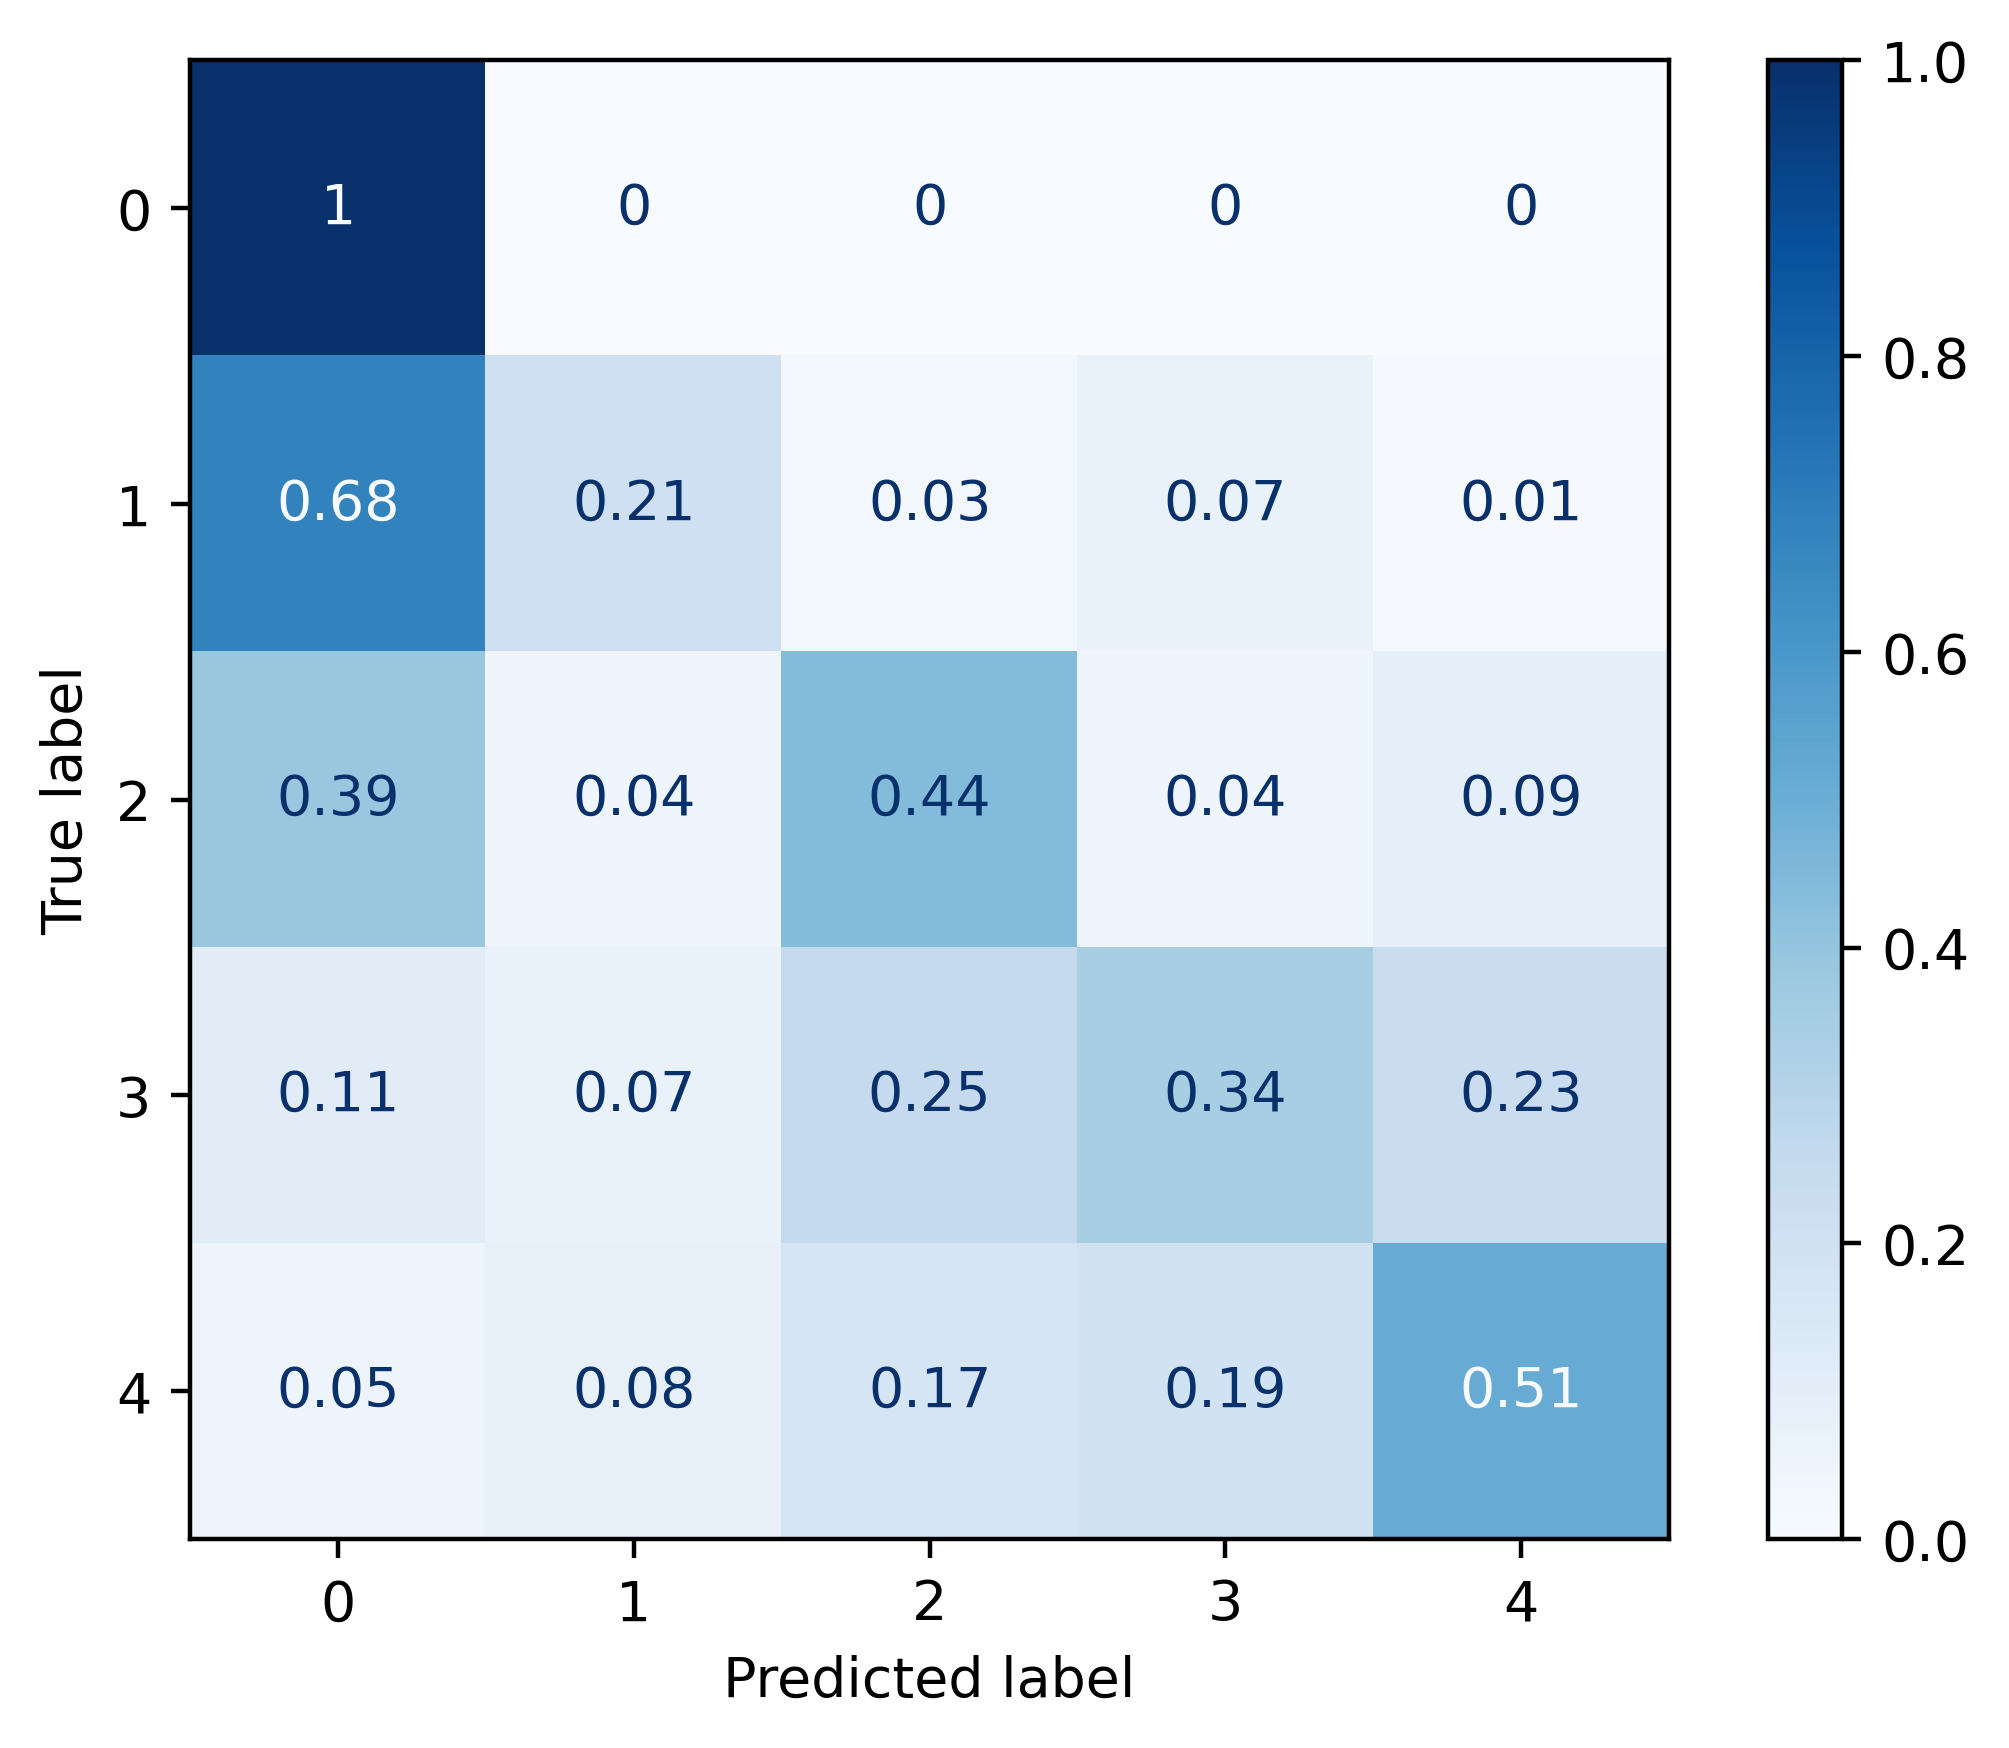
\includegraphics[scale=0.8]{img/resnet18_confusion_matrix_pretrained.png}
		\caption{Confusion matrix of ResNet-18 (pretrained).}
		\label{resnet18-pretrained-confusion-matrix}
	\end{figure}

	\begin{figure}[H]
		\centering
		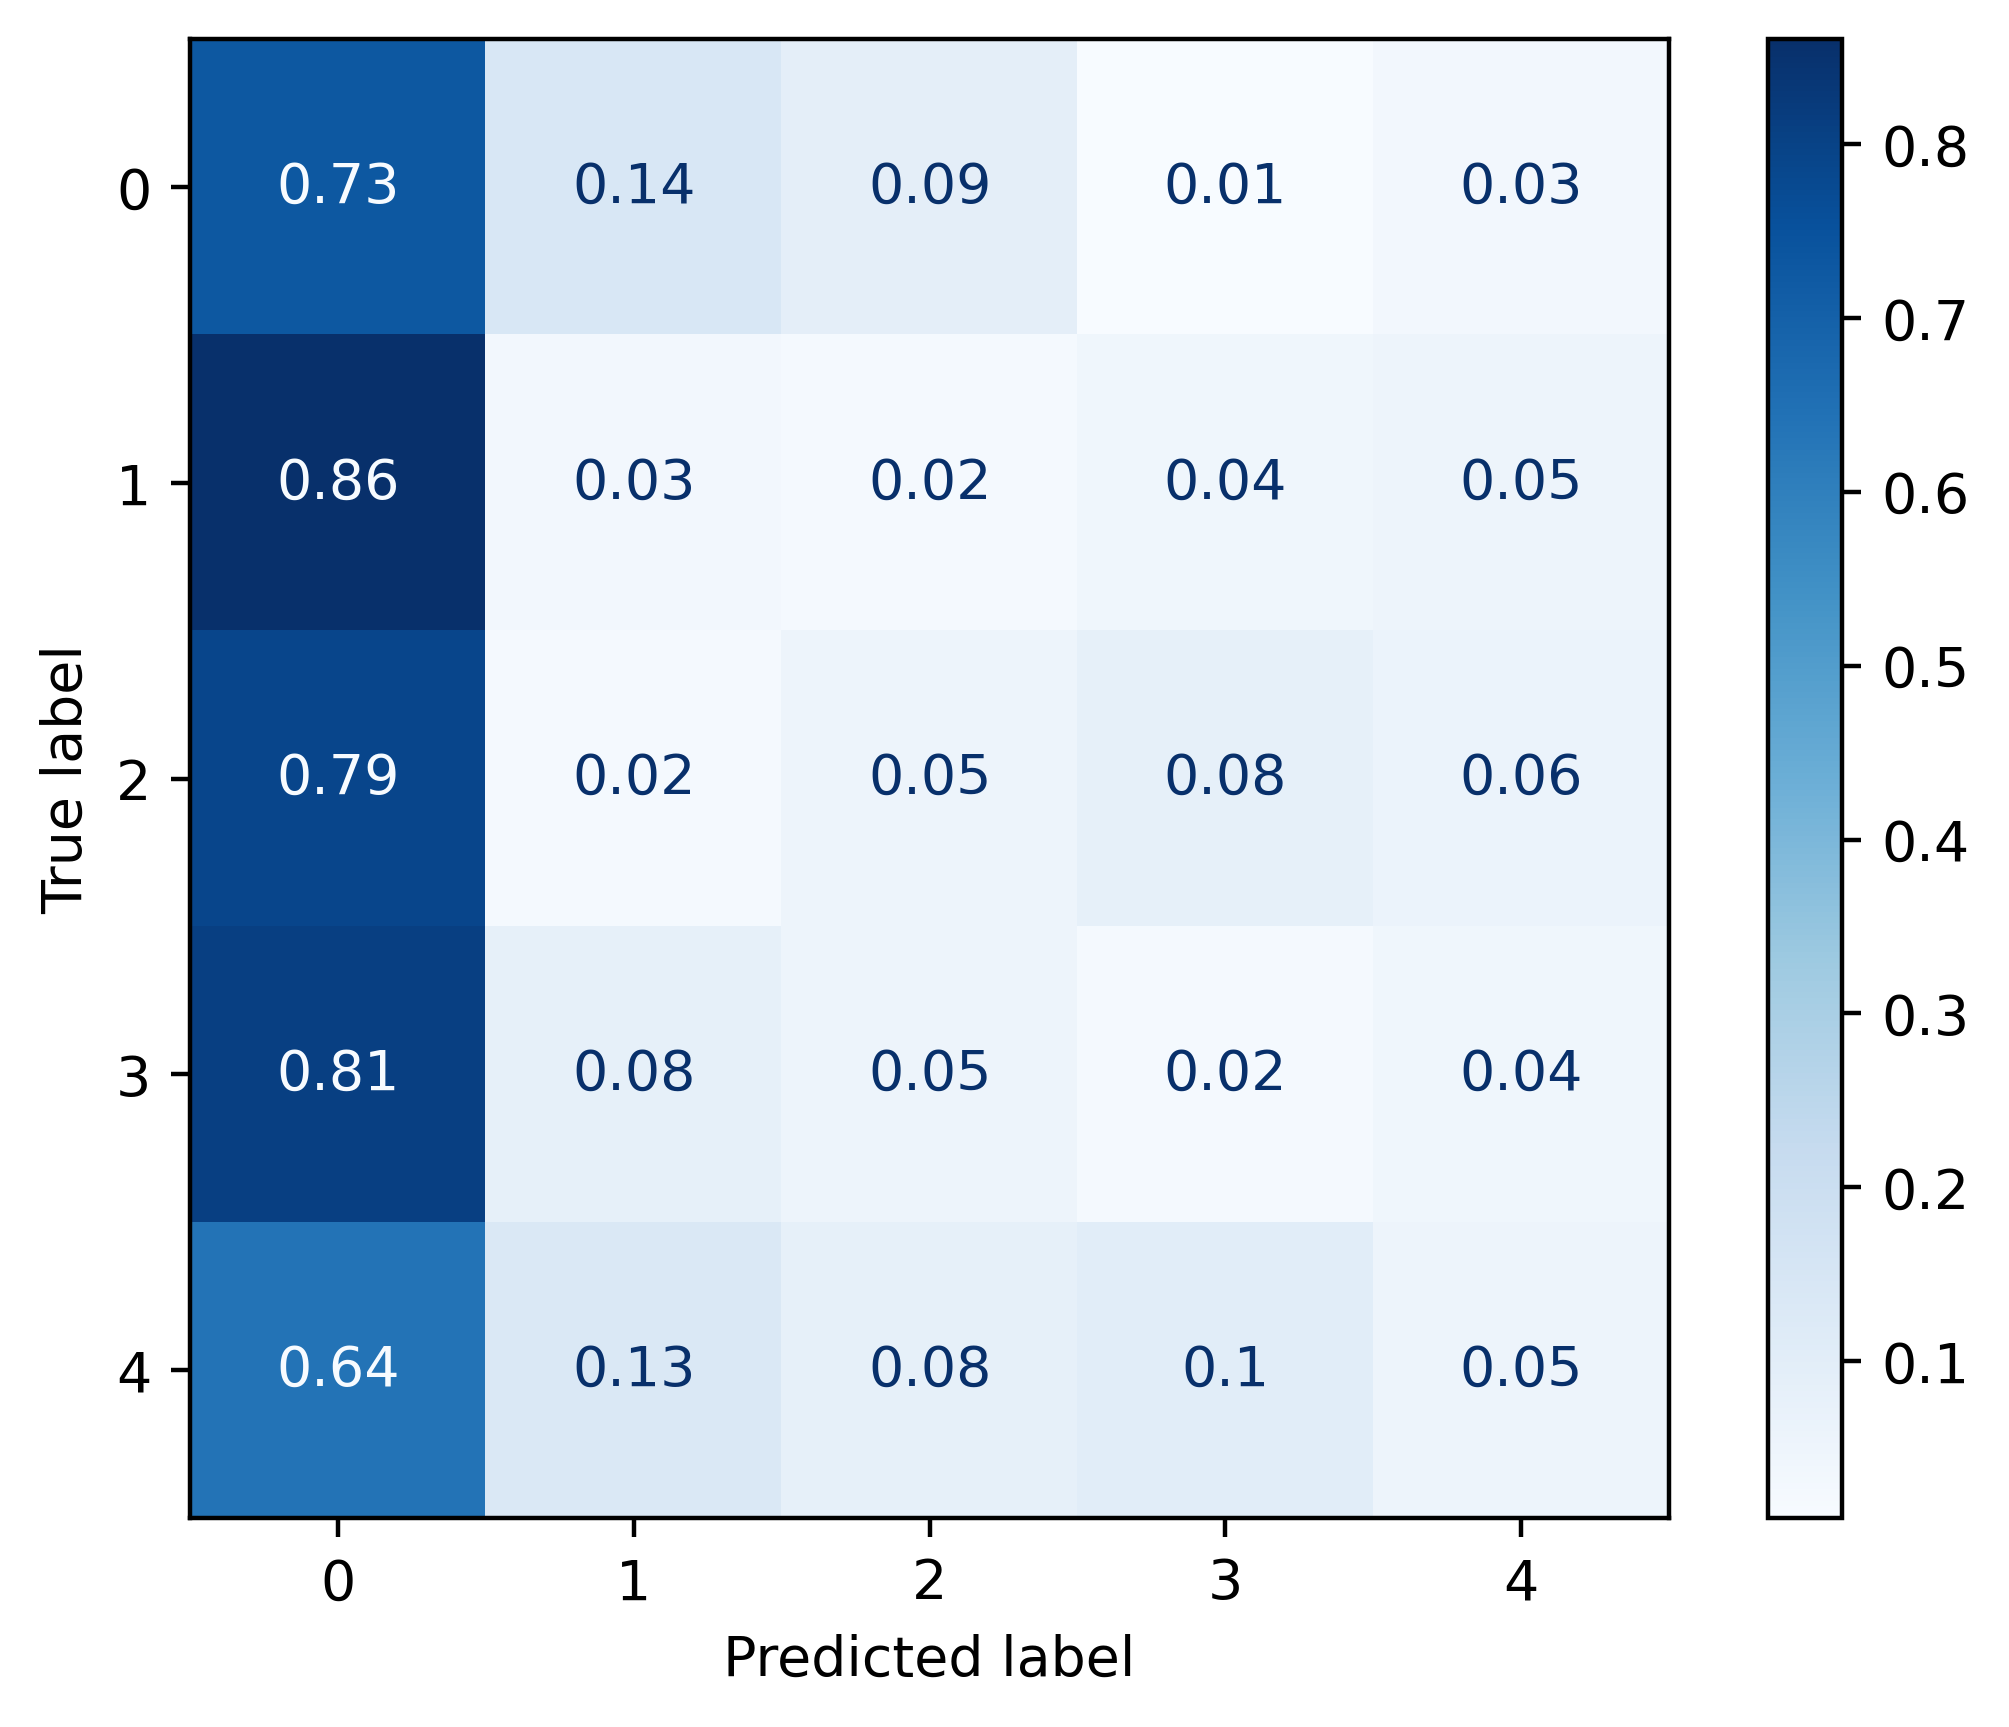
\includegraphics[scale=0.8]{img/resnet50_confusion_matrix_mine.png}
		\caption{Confusion matrix of ResNet-50 (without pretrained).}
		\label{resnet50-mine-confusion-matrix}
	\end{figure}
	\begin{figure}[H]
		\centering
		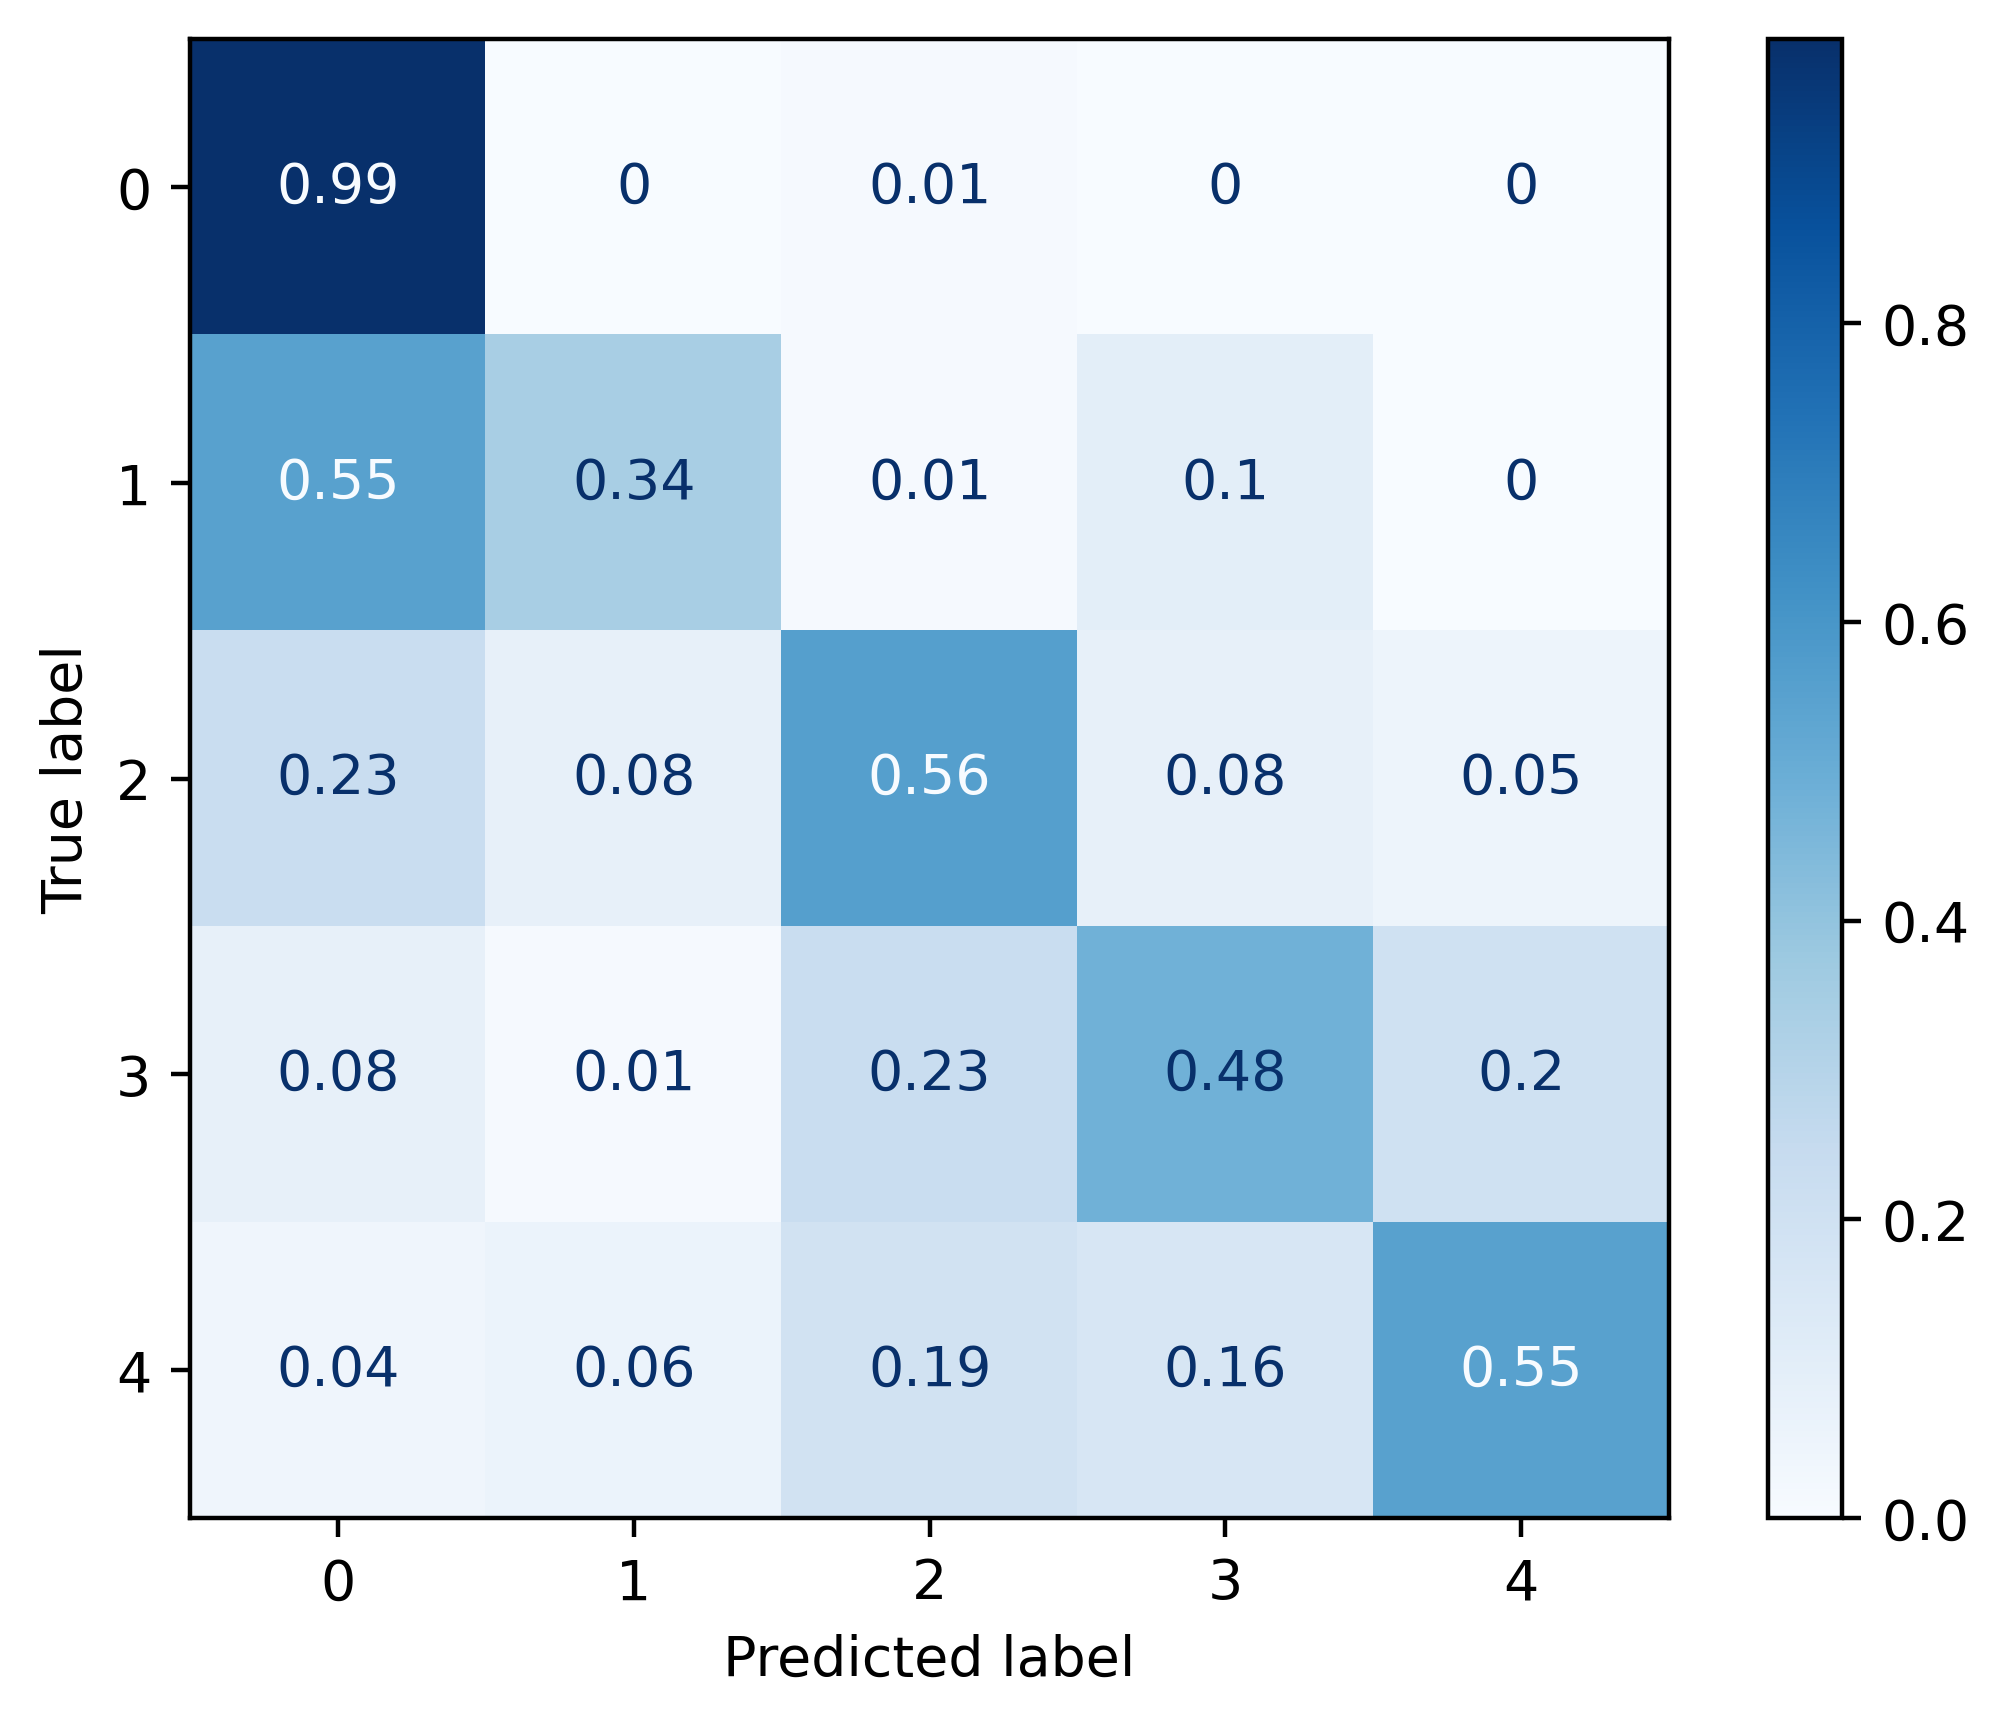
\includegraphics[scale=0.8]{img/resnet50_confusion_matrix_pretrained.png}
		\caption{Confusion matrix of ResNet-50 (pretrained).}
		\label{resnet50-pretrained-confusion-matrix}
	\end{figure}
